\chapter{Literature Review}
\label{chap:literature_review}

This chapter exposes some of the works whose content is relevant to
the context of this dissertation. Section
\ref{sec:privacy_pervasive_computing} begins by explaining the concept
of location privacy in pervasive computing and it's importance. It then follows
with the presentation of some of the approaches already used in the
field of pervasive computing that deal with this topic. Lastly, Section
\ref{sec:algorithms_and_data_structures} provides some background to
the algorithms and classic data structures used in our approach to ensure
privacy.

\section{Location Privacy in Pervasive Computing}
\label{sec:privacy_pervasive_computing}

As location based services become more popular and compelling, there
is an increasing temptation to give away location data. However, along
with this enticement comes an increasing concern about location
privacy. Before going into any further details, it is important to
correctly understand what location privacy is.

\subsection{Definition of Location Privacy}
\label{sec:definition_privacy}

Beresford and Stajano ~\cite{1186725} define location privacy as:
\begin{quotation}
  ``...the ability to prevent other parties from learning one's
  current or past location.''
\end{quotation}
Their definition implies that a person whose location is being
monitored must be able to control who has access to that information.
It also acknowledges that both past and present information, regarding
location, is important. While current location information might
enable an attacker to find out where a person is, past data can allow
him/her to discover who the person is and where does she live/work,
and even predict future locations.

According Duckham and Kulik~\cite{duckham2006location} location
privacy is:
\begin{quotation}
  ``a special type of information privacy which concerns the claim
  of individuals to determine for themselves when, how, and to what
  extent location information about them is communicated to others.''
\end{quotation}
Their definition is based upon Westin's~\cite{westin1968privacy}
definition of information privacy:
\begin{quotation}
  ``the claim of individuals, groups or institutions to determine for
  themselves when, how and to what extent information about them is
  communicated to others.''
\end{quotation}
Duckham and Kulik's definition captures several aspects about
location information and the way it can be shared:
\begin{itemize}
\item When: A user might have different concerns regarding her present
  and past locations. For instance, the user may not care as much
  about revealing her past locations as it does about its present
  location.
\item How: A user might be comfortable with manual location requests
  from her friends, however she may not want to have her friends
  alerted automatically when she enters a casino or a bar.
\item Extent: A user might prefer to have her location reported as an
  ambiguous region rather than as a precise point.
\end{itemize}
These different aspects are the topic of many different
computational schemes for protecting the privacy of the users.
Examples of such schemes are the use of pseudonyms instead of actual
names, the deliberate addition of noise to the location data or the use
of regions for location reporting instead of specific points.

\subsection{Related Work}
\label{sec:lp_related_work}

% In the context of ubiquitous computing, there are already several
% techniques aimed at ensuring the privacy of data regarding the
% location of the users.

In the past few years there has been an exponential increase in the
number of mobile devices (smartphones, laptops, tablets). Many of
these devices come equipped with several types of sensors
(accelerometer , gyroscope, thermometer, GPS) as well as communication
interfaces (Bluetooth, WiFi). Their pervasiveness associated with
their capabilities make them viable building blocks for urban
pervasive infrastructures~\cite{kostakos2009understanding}. Associated
with the increasing number of mobile devices is the popularity growth
of Location-Based Services (LBS)\cite{zickuhr2012three}. LBSs
determine the location of the user by using one of several
technologies for determining its position, and then use the location and
other information to provide personalized applications and
services~\cite{zibuschka2011location}. There are however privacy risks
that stem from the use of such services.
PleaseRobMe\footnote{www.pleaserobme.com} was created to raise awareness
for the risks of sharing location information. Combining information
from FourSquare\footnote{www.foursquare.com} and
Twitter\footnote{www.twitter.com} it demonstrates how easy it is to
infer that someone is not at home. Despite the existence of reports
linking the sharing of location information with the occurrence of
robberies~\cite{Grove:2009:Online,Dybwad:2009:Online}, there are
several research works which show that most people put little value on
their location privacy~\cite{ahern2007over,colbert2001diary,
  Cvrcek:2006:SVL:1179601.1179621,kaasinen2003user}. However, this
lack of concern by the users of LBSs is usually a consequence of lack
of awareness. In \cite{kaasinen2003user} the author notes that,
despite not being worried about the privacy issues arising from location aware
services, most of the users were not aware they could be located while
using those services. On the other hand, the work in
\cite{Cvrcek:2006:SVL:1179601.1179621} shows that the Greeks demanded
a higher price for their location data when compared with the other EU
countries. According to the author, this might have been a consequence
of the eavesdropping scandal involving the wiretap of Greek
politicians that took place 2 months before the survey. This might
indicate that people value their privacy the most when faced with
consequences from the lack of it. Sharing location data at such a
large scale like we see today is relatively new. As a consequence, the
effects on user privacy are not fully understood
yet \cite{Terrovitis:2011:PPD:2031331.2031334}.

According to Duckham and Kulik's survey in \cite{duckham2006location},
there are four commonly used methods for ensuring location privacy:
\begin{itemize}
\item Regulatory strategies: comprised by government rules on the use
  of personal information.
\item Privacy Policies: trust-based mechanisms established
  between individuals and whomever is receiving their location data.
\item Anonymity: Disassociation between the individual's personal
  information and individual's actual identity. Usually obtained
  through the use of pseudonyms, ambiguity and cloaking.
\item Obfuscation: degradation of the quality of the location data.
\end{itemize}

From these four methods, we will concentrate in the last two because
they are the most relevant in the context of this dissertation.

\subsubsection{Anonymity}
\label{sec:privacy_anonimity}

The use of pseudonyms is perhaps the most obvious way to achieve
anonymity. However, using same pseudonym for a long time makes it is
easy for an attacker to gather enough history on an individual to
infer their habits or true identity. To try to mitigate this issue,
Beresford and Stajano in \cite{1186725} proposed an idea which relied
upon pseudonym exchange. They introduced two new concepts: \emph{mix
  zone} and \emph{application zone}. A \emph{mix zone} for a group of
people is defined as the maximum contiguous area where none of the
group's users exchanges information with a LBS. This prevents the
users' data from being accessed by the LBS providers. By contrast, an
\emph{application zone} is defined as an area where at least one of
the users exchanges data with a LBS. By switching her pseudonym to a
new unused one when entering a \emph{mix zone}, the user ensures that
there is no way for a LBS provider to distinguish between her and the
other users who were in that zone. This means that there is no way for
attackers to link people going into the mix zone with the ones that
come out of it.

Based on a different concept, \emph{k-anonymity} (introduced by
Samarati and Sweeney in~\cite{samarati1998protecting}) Gruteser and
Grunwald~\cite{gruteser2003anonymous} were the first to investigate
anonymity as a method to attain location privacy. According to them, a
subject is considered to be k-anonymous with regard to location
information, if and only if she is indistinguishable from at least
$k-1$ other subjects with respect to a set of
\emph{quasi-identifier} attributes. Bigger values of $k$ correspond to higher degrees of
anonymity. They proposed a middleware architecture and an algorithm
capable of adjusting location information resolution in spacial and/or
temporal dimensions in order to comply with a specific
\emph{k-anonymity} requirement. When a client requests a service,
their algorithm calculates a \emph{cloaking box/region} that contains
that client along with at least $k-1$ other users. That box is then
used as the client's location to request the service. If that box's
resolution is to coarse for some services, temporal cloaking can be
applied by delaying the user's service request. When more users come
near the client, a smaller cloaking region can be computed. This concept
has since been explored and improved in other scientific works.

Geddik and Liu's
\emph{ClickCloak} algorithm
~\cite{gedik2005location,gedik2008protecting} allows each user to
define her own minimum acceptable value for $k$ ($k_{min}$), as well
as the maximum acceptable values for temporal and spacial resolution.
Furthermore, they created an efficient message perturbation engine
capable of performing location anonymization of users' requests.
This is accomplished by removing the users' identities from the
requests and with the use of spatiotemporal obfuscation of the
location information.

Mokbel et al. in~\cite{mokbel2006new} use the \emph{k-anonymity}
concept as well.  They presented the Casper framework which consists of
two main components, a location anonymizer and a privacy-aware query
processor.  The location anonymizer blurs the location information
about each user according to that user's defined preferences (minimum
area $A_{min}$ in which she wants to hide and minimum value for
$k$). The query processor tunes the functionality of traditional
location-based databases to be privacy-aware. It does so by returning
cloaked areas instead of exact points when queried for location
information.

Unlike the previous \emph{k-anonymity} based approaches that require a
centralized trusted server (Anonymizer) in order to compute the cloaking
regions, Ghinita et al. in ~\cite{ghinita2007prive} use a
decentralized peer-to-peer approach. This fixes two issues inherent to
the centralized server approach:
\begin{itemize}
\item Fault Tolerance -  the
anonymizer is a single point of failure and the system cannot work
without it.
\item Security - all requests must go through the anonymizer, so in
  case it becomes compromised it would result in a serious security
  threat.
\end{itemize}

Their distributed protocol called PRIVÉ supports decentralized query
anonymization with load balancing and fault tolerance. In PRIVÉ, for a
user to be considered trustworthy and participate in the network, she
needs a trust certificate obtained from a Certification Server. Users
in the network trust each other and communicate using a structured
peer-to-peer network. Users are grouped into clusters according to
their location. Each cluster has a leader which is recursively grouped
with other leaders to form other clusters with different leaders, just
like a B-Tree structure. This allows each user to create it's own
cloaking region by using information from other nearby users.
Furthermore, PRIVÉ also ensures \emph{reciprocity} in the creation of
cloaking regions. A cloaking region with $k$ users satisfies
reciprocity only if that same cloaking region is generated for each of
users. This means that an attacker cannot use \emph{minimality} attacks
\cite{wong2007minimality}, i.e., it cannot infer which user is the
source of the request with a probability bigger than $\frac{1}{k}$.

\subsubsection{Obfuscation}
\label{sec:Obfuscation}

Obfuscation based techniques usually degrade the ``quality'' of the
information in order to provide privacy protection. Even tough this may
seem comparable to what \emph{k-anonymity} based techniques do, there is a
key difference: obfuscation based techniques allow the actual identity
of the user to be revealed (thus making it suitable for applications
that require authentication or offer some sort of personalization
\cite{langheinrich2001privacy}).

Duckam and Kulik
\cite{duckham2005formal} were the ones who introduced the idea of
obfuscation for location privacy. They talk about three distinct types of
imperfection that can be present in spacial information:
\begin{itemize}
\item Inaccuracy - lack of correspondence between information and
  reality. E.g. ``Braga is in Spain''
\item Imprecision - lack of specificity in the information. E.g.
  ``Braga is in Europe''
\item Vagueness - special type of imprecision that concerns the
  existence of indeterminate borderline
  cases~\cite{duckham2001formal}. E.g. ``Braga is in western Europe''.
  This is a vague statement since there is no clear definition about
  the borders of western Europe.
\end{itemize}

Any of these types of imperfection can be used to obfuscate an
individual's location. In this particular case, the authors use
imprecision to degrade the quality of the location information.
They adopt a discrete model for space representation through the use of
graphs. Geographic locations are modeled as a set of vertices $V$, and
the connectivity or adjacency between them is modeled as a set of
Edges $E$. A user's location is represented through a
vertex $l \in V$. Obfuscation is provided through the use of a group
of vertices $O$ such that $l \in O$ and $O \in V$, where for every
element $o \in O$, $o$ is \emph{indiscernible} from $l$. The larger
the set $O$, the less information is being revealed and therefore, the
greater is that individual's privacy. The set $O$ is used by their
algorithms to negotiate the balance between an individual's location
privacy and that individual's need for quality services. The more
information an individual is willing to reveal the higher the quality
of information he can be provided with.

Another example of an obfuscation based approach was shown by
Ardagna et al. in ~\cite{ardagna2007middleware} and later improved in
\cite{ardagna2007location, ardagna2011obfuscation}. Their obfuscation
process allows users to express their privacy preferences using
another concept of theirs called \emph{relevance}. Relevance is a
value in the range $]0,1]$ and it represents the relative accuracy
loss in location measurement. It tends to 0 when the location
measurement is highly inaccurate and it is equal to 1 when the
location measurement achieves the best accuracy allowed by the
location technique in use. The higher the relevance the lower will be the
location privacy. Moreover, they define a set of basic
\emph{obfuscation operators} that are used to modify location
measurements. These operators can be further composed in order to
increase robustness against deobfuscation attacks and are
randomly selected and applied to the user's measured location ensuring
that the selected relevance value holds. This solution allows users to
abstract from both the obfuscation operators and the sensing
technology (Bluetooth, Wifi, GPS).

There are other examples of obfuscation approaches that are not only
oriented to location data but to the degradation of data in general
\cite{anciaux2008instantdb,heerde2006data}. In these approaches,
privacy is obtained through the generalization of the information.
This procedure is done resorting to generalization trees
\cite{anciaux2008instantdb} or generalization graphs
\cite{heerde2006data}. These structures contain the sets of rules to
be applied in the generalization process. The application of these
rules depends on the Life Cycle Policy (LCP). A LCP consists of the
set of transitions between the generalization structures'
branches/vertexes as well as the events that trigger them. The biggest
challenge in this type of approaches is the difficulty associated with
the construction of the sets of rules and the generalization
structures.

% for self-protection, it is natural and necessary for a user to
% withhold her true identity when requesting an LBS. However, simply
% using a pseudonym, or not using any identifier at all, is not
% sufficient. This is due to the fact that a user’s location itself may
% be correlated with restricted spaces such as house and of- fice to
% reveal her real-world identity. For example, if a location belongs to
% a private property, then the adversary can derive that the user is
% most likely the owner of the property. A single loca- tion sample may
% not be linked directly to a particular user, but the accumulation of a
% time-series sequence of her location samples will eventually reveal
% her identity \cite{gruteser2005anonymity, xu2007location}. Once the
% user is identified, all her visits may be disclosed.

\section{Algorithms and data structures}
\label{sec:algorithms_and_data_structures}
In our work, we tested how the usage of stochastic summarizing
techniques fared as an approach to some privacy preserving
scenarios. These techniques provide both the concepts we talked about
in the previous section, anonymity and obfuscation. Being
non-deterministic summarizing techniques, they degrade the quality of
information in such a way that does not allow the recreation of the
original data, thus the obfuscation property. On the other hand, by
relying on hash functions to create pseudonyms, they afford anonymity.

This section briefly explains the algorithms
and data structures that were used in both the Gate Counting
(Chapter~\ref{cha:gate-counting}) and Causality Tracking
(Chapter~\ref{cha:causality-tracking}) scenarios.

\subsection{Hash Sketches}
\label{sec:hash_sketches}

Hash Sketches are a simple probabilistic data structure used to obtain
the number of distinct elements in multisets. There are several
variants of Hash Sketches. Despite being different, all the discussed
variants have at least one bit array and use some kind of
hash function to map elements from the multiset to positions in the
bit array(s). The main idea is to use an hash function to
randomize data and create what closely resembles to an uniform and
independent binary data structure. This pragmatism is justified by
Knuth \cite{knuth1998art}:
\begin{quotation}
``It is theoretically impossible to define a hash
function that creates random data from non-random data in actual
files. But it is not difficult to produce a pretty good imitation of
random data.''
\end{quotation}
This binary data structure is then used as input to an
\emph{estimator} function that returns an \emph{estimation} of the
number of distinct elements in the multiset, it does not return exact
results. The estimator performs some tests on the hashed
binary data comparing the obtained results with the ones that would be
expectable using probabilistic analysis. Finally, it infers an estimate
for the number of distinct elements.

In Hash Sketches, the same element is always mapped to the same
position(s) in the binary array(s). That is the reason why this
algorithm is only suitable to estimate the number of distinct
elements, i.e. the cardinality of the support set of a multiset. The
support set is a subset of the multiset with all the distinct elements (no
repetitions).

Due to their probabilistic nature, Hash Sketches also have a smaller
memory footprint than the one that would be needed in a deterministic
approach. Hash Sketches also have the ability to estimate the number
of different elements incrementally and in a single pass over the
multiset. This enables them to provide on-the-fly estimates in
scenarios where there is a constant flow of data.

It is also worth noting that all the ``observables'' i.e. bit
array(s) used by the Hash Sketches algorithms below, are
duplicate and order insensitive. This means that, neither the order in
which elements are inserted, nor the insertion of repeated elements
affect the output of the estimator functions.

In the Gate Counter Scenario (Chapter \ref{cha:gate-counting}), we
tested several versions of sketches: LogLog Sketches
\cite{Durand:2003tc}, HyperLogLog Sketches \cite{Fusy:2007um}, Linear
Counting Sketches \cite{Whang:1990uh}, Robust-In Network Aggregation
Linear Counting Sketches (RIA-LC)
\cite{Fan:2008wl,YaoChungFanArbeeLPChen:2010to} and Robust In-Network
Aggregation Dynamic Counting Sketches (RIA-DC)
\cite{YaoChungFanArbeeLPChen:2010to}.

\subsubsection{LogLog Sketches}
\label{sec:loglog-sketches}
LogLog Sketches \cite{Durand:2003tc} are similar to the Probabilistic
Counting with Stochastic Averaging (PCSA) algorithm presented in
\cite{Flajolet:1985wd} since both use several small bit arrays (called
buckets) instead of a single bit array. This concept was introduced in
\cite{Flajolet:1985wd} under the name \emph{stochastic averaging} and
its purpose is to reduce the \emph{variance} of the estimates, thus
improving their accuracy. The main difference between PCSA and LogLog
Sketches is that the latter consume a lot less memory at the expense
of some accuracy. To create a LogLog sketch, one needs to know the
number of distinct elements it will hold, or at least an upper bound
for that number. This number and the desired accuracy are the
two design parameters for this algorithm. Having defined those, $m$
buckets are created and initialized to $0$. Each bucket has a size
close to $log(log(N_{max}))$ (hence the name LogLog Sketches), being
$N_{max}$ the maximum number of distinct elements the sketch can hold.
Given the hash code for element $e$, $hs(e)$, let $\mathfrak{R}_e$
denote that code without the first $k=log_2(m)$ elements and $\rho(x)$
a function that returns the index (starting at 1) of the leftmost $1$
bit in $x$, e.g. $\rho(1\ldots)=1,\ \rho(0001\ldots)=4$. To insert an
element $e$ in the Sketch, the first $k$ bits of the element's hash
code are used to pick one of the buckets, lets assume it was bucket
$b_1$. Its content is updated as follows,
$b_1=max(b_1,\rho(\mathfrak{R}_e))$. The values stored in the various
buckets are the ones used by the estimator function to provide a
number for the cardinality of the support set.

\subsubsection{HyperLogLog Sketches}
\label{sec:hyperloglog-sketches}
HyperLogLog Sketches \cite{Fusy:2007um} are an improvement over LogLog
Sketches. In both algorithms, greater accuracy can be obtained at the
cost of bigger space requirements and lower space requisites can be
bought at the expense of reducing the accuracy. However, when using the same
number of bits as in LogLog Sketches, HyperLogLog Sketches is able to
provide more accurate results. According to the authors, this
improvement stems from the use of \emph{harmonic means} instead of
\emph{geometric means} in the estimator function. The key concept
behind both these algorithms is that using a good hash function, it is
expected that only $N/2^y$ distinct elements have a $\rho$ value equal
to $y$, where $N$ is the number of distinct elements in the multiset
(e.g. $\rho(x)=1$ in $50\%$ of the cases, $\rho(x)=2$ in $25\%$ of the
cases, $\rho(x)=3$ in $12.5\%$ of the cases, \ldots). Figure
\ref{fig:hyperloglog_sketches} shows the behavior of these algorithms,
but for ease of representation instead of small bit arrays it uses
integers to represent the buckets.
%Insertion works as follows:
% \begin{enumerate}
% \item Starting from left to right (it could be done from right to
%   left, as long as we stay coherent), let $i$ be the first
%   index whose bit is set to 1. In case of ``ELEM1'', $i=4$.
% \item Counting on the same direction as the first step and
%   assuming indexes start at $1$, set bucket$[i]=1$. In case of
%   ``ELEM1'', we set bucket$[4]=1$.
% \item Repeat the above steps for all elements.
% \end{enumerate}
\begin{figure}[htb]
  \centering
  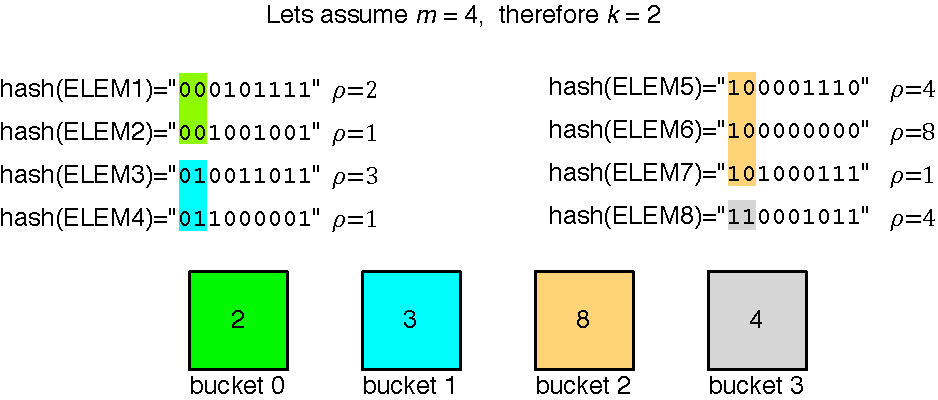
\includegraphics[width=\textwidth]{images/hll_sketches.pdf}
  \caption{Insertion of elements in a (Hyper)LogLog Sketch}
  \label{fig:hyperloglog_sketches}
\end{figure}

\subsubsection{Linear Counting Sketches}
\label{sec:line-count-sketch}
Linear Counting (LC) Sketches \cite{Whang:1990uh}, on the other hand,
use a single bit array/sketch with size $m$. This sketch is
initialized with $0$s. When an item $i$ is to be inserted, its hash
value $h_i$, is used to calculate an index within the sketch
($mod(h_i,m)$), which is then set to $1$. To calculate the estimate of
the number of different items, the algorithm uses the fraction of
empty sketch entries ($V_n$). In order to obtain this value, it counts
the number of empty sketch entries (the number of $0$ entries in the
sketch) and divides it by the total size of the sketch. The key
concept behind LC Sketches is that for a uniformly distributed hash
function, it is expected for the fraction of zero bits in the sketch
to be inversely proportional to the number of distinct elements in the
multiset. LC Sketches' name comes from their linear space complexity
$O(N_{max})$ (where $N_{max}$ is the maximum number of different
elements that the sketch can hold), i.e. their size grows linearly
with the number of distinct elements that can be hold. Compared to
(Hyper)LogLog Sketches, LC Sketches' space complexity is a drawback,
specially for multisets with large numbers of distinct elements.
However, LC Sketches are easier to implement and also provide better
estimates in multisets with a small number of distinct elements.
Figure \ref{fig:lc_sketches} shows a LC Sketch with size $m=16$, after
the insertion of 4 elements, $V_n=0.75$. Notice that ``ELEM4'' is
inserted in index $i=12$ because that is the remainder of the integer
division of 44 over 16.

\begin{figure}[htb]
  \centering
  \includegraphics[width=\textwidth]{images/lc_sketch.pdf}
  \caption{Linear Counting Sketch after the insertion of 4 elements}
  \label{fig:lc_sketches}
\end{figure}

\subsubsection{Robust In-Network Aggregation Linear Counting Sketches
  and  Robust In-Network Aggregation  Dynamic Counting Sketches}
\label{sec:robust-netw-linear}
Both Robust In-Network Aggregation Linear Counting Sketches (RIA-LC)
\cite{Fan:2008wl,YaoChungFanArbeeLPChen:2010to} and Robust In-Network
Aggregation Dynamic Counting Sketches (RIA-DC)
\cite{YaoChungFanArbeeLPChen:2010to} are based on LC Sketches. RIA-LC
sketches are a slightly improved version of Linear Counting Sketches.
They are very similar in the way they work, however RIA-LC Sketches
are less prone to the overflow problem that occurs in LC Sketches when
all the bits in the sketch are set to $1$.

One of the major issues with all of the previous algorithms is the
merge operation. All of them allow the merging of several sketches of
the same type to obtain an aggregate count of the number of distinct
elements. However, all the sketches to be merged must be similar (same
size/accuracy). Furthermore, each of them has to be big enough to hold
the aggregate number of distinct elements. For instance, given two
sketches with no overlap between their elements, with $200$ and
$10000$ distinct elements, if we plan on computing their aggregate
then each sketch must be big enough to hold at least $10200$ elements.
RIA-DC sketches don't suffer from this issue. They have the ability to
merge sketches of different sizes. However, this ability comes with a
price. RIA-DC Sketches assume that elements belonging to different
sketches do not overlap, meaning that if we merge two
different RIA-DC sketches with elements in common, those elements will
be counted twice in the final aggregate.

\subsection{Bloom Filters}
\label{sec:bloom_filters}

Bloom Filters (BFs) were created in 1970 \cite{Bloom1970} by Burton
Howard Bloom. They are a simple and space efficient data structure for
set representation where membership queries are allowed. Bloom Filters
allow false positives but do not allow false negatives, i.e, when
querying a Bloom Filter about the existence of an element in a given
set, if the answer is no, then the element is definitely not in the
set, but if the answer is yes, the element might be in the set.

A Bloom Filter for representing a set of $n$ items $S =
\{x_1,x_2,x_3,...,x_n\}$ is traditionally implemented using an array
of $M$ bits, all initially set to 0. Then, $k$ independent hash
functions are used $\{h_1,h_2,...,h_k \}$, each one mapping the
element of the set into a random number uniformly distributed over the
range $\{1,...,M\}$. For each element $x$ of the set ($x \in S $) the
bits of the positions $h_i (x)$ are all set to 1 for $1 \leq i \leq
k$. A location can be set to 1 multiple times. Due to the independence
of the hash functions, nothing prevents collisions in the outputs. In
extreme cases it is possible to have $h_1(x) = h_2(x) = ... = h_k(x)$.
To prevent this, we use the variant of Bloom Filters presented in
\cite{Chang04approximatecaches} which partitions the $M$ bits among
the $k$ hash functions, creating $k$ slices of $m = M/k$ bits. This
ensures that  each item added to the filter is always described by $k$ bits.
Given a Bloom Filter $BF_S$, checking if an element $z \in BF_S$,
consists in verifying whether all $h_i(z)$ are set to 1. If they
aren't, then $z$ is definitely not present on the filter. Otherwise,
if all the bits are set to 1, then it is assumed that $z$ belongs to
$BF_S$ although that assumption might be wrong. This false positive
probability exists because the tested indices might have been set by
the insertion of other elements. Figure \ref{fig:bloom_filter}
illustrates such an example.
\begin{figure}[htb]
  \centering
  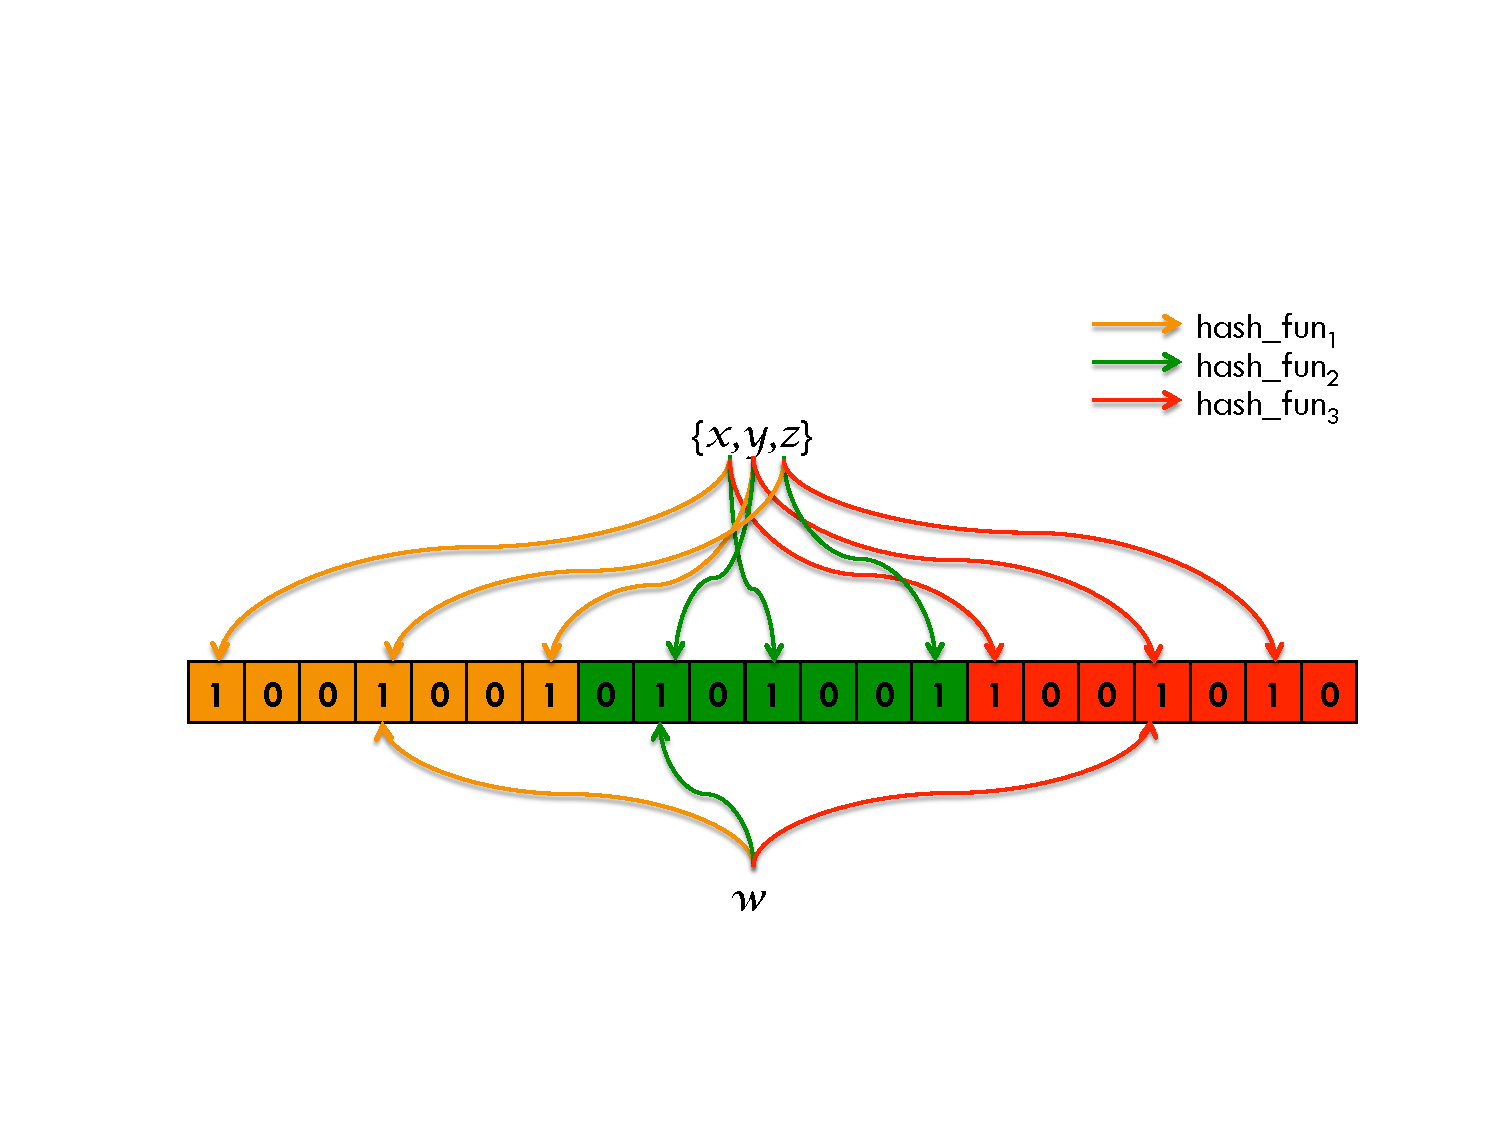
\includegraphics[width=\textwidth]{images/bloom_filter.pdf}
  \caption{ Bloom Filter with $k=3$, $M=21$ and $m=7$, containing
    elements $\{x,y,z\}$. Querying for the presence of element $w$
    yields a false positive.}
  \label{fig:bloom_filter}
\end{figure}

The false positive probability $P$
can be obtained using equation (\ref{eq:false_positive}), where $p$ is
the ratio between the number of set bits in the slice and the slice
size $m$. The fill ratio $p$ can be obtained through equation
(\ref{eq:fill_ratio}).

\begin{equation}
  \label{eq:false_positive}
  P = (1-p)^k
\end{equation}

\begin{equation}
  \label{eq:fill_ratio}
  p = 1-\left(1-\frac{1}{m}\right)^n
\end{equation}

Furthermore, given a maximum false positive probability $P$, and the
number $n$ of distinct elements to store, equations
(\ref{eq:optimal_hash_number}) and (\ref{eq:optimal_slice_size}) can
be used to estimate the optimal number of bits required by a Bloom
Filter to store those $n$ elements, $M=m*k$.

\begin{equation}
  \label{eq:optimal_hash_number}
  k = log_2\left(\frac{1}{P}\right)
\end{equation}

\begin{equation}
  \label{eq:optimal_slice_size}
  m = \frac{n*|lnP|}{k*(ln2)^2}
\end{equation}

\subsubsection{Counting Bloom Filters}
\label{sec:count-bloom-filt}

Counting Bloom Filters (CBFs) were presented in
\cite{Fan98summarycache:} although they were only given this name
later in \cite{Mitzenmacher:2002:CBF:581876.581878}. They were
introduced in order to allow the deletion of elements from the Bloom
Filters. Suppose that we have a set that changes over time, where
elements are inserted and deleted. The insertion of elements can be
easily done using a normal Bloom Filter, hash the element $k$ times
and set the bits to 1. Unfortunately the delete operation cannot be
accomplished simply by reversing the process. The resulting positions
from the hash functions cannot be set to 0, because each position may
be hashed by some other element from the set.

In a Counting Bloom Filter, each position is a small counter rather
than a single bit. When an item is inserted the corresponding counters
are incremented, and when the item is deleted the same counters are
decremented. We just have to choose sufficiently large counters, in
order to avoid counter overflow.

\subsubsection{Scalable Bloom Filters}
\label{sec:scal-bloom-filt}

As we have seen, Bloom Filters provide space-efficient storage of sets
at the cost of a probability of false positives on membership queries.
A conservative approach is usually chosen when filters are created
because in case the number of elements stored surpasses the original
number that the filter was supposed to hold, the false positive
probability starts to increase rapidly. That conservative approach
usually leads to filters orders of magnitude larger than needed and
consequently to wasted space. To tackle this issue, Almeida et
al. \cite{Almeida2007} introduced the concept of Scalable Bloom Filters
(SBF), a variant of Bloom Filters that can adapt dynamically to the
number of elements stored while respecting a maximum false positive
probability, which is chosen in the beginning. SBF are a mechanism that
adapts to growth of sets using a series of classic Bloom Filters of
increasing sizes and tighter false positive probabilities. When the
filters get full, a new one with $size = previous\ size*growth\ rate$
and tighter false positive probability is made. To check for the
presence of an element, one has to query all filters.

\subsection{Vector Clocks}
\label{sec:vector_clocks}

Broadly speaking, a distributed system consists in a set of processes
connected through a network. Each of these processes' internal state can only
change through the occurrence of events. There are 3 kinds of events: message
sending, message reception and state transition events deriving from the
normal execution of the process. In a distributed system, processes can only
communicate using message passing as there is no shared memory. In this
context and considering the ordering of events in an asynchronous model (since
no assumptions should be made about timing), several strategies to cope with
this asynchronicity were devised. One of the most prominent is vector clocks.

In order to better understand how Vector Clocks work, we must first comprehend
the concept of causality.  Causality is a relation through which we can connect
two events, a first event (known as the \textit{cause}) and a second one (the
\textit{effect}).

In the context of Distributed Systems, causality is expressed using the
\textit{happens-before} relation \cite{Lamport:1978} denoted by the
$\rightarrow$ symbol. For instance, given 2 events, $x \rightarrow y$, reads
as $x$ happened-before $y$, and means $y$ might be a consequence of
$x$.

The \textit{happens-before} relation has the following properties over any given event:
\begin{itemize}
\item $\forall a,b,c$ if $a \rightarrow b$ and $b\rightarrow c$, then $a
  \rightarrow c$ (transitivity);
\item $\forall a, a \nrightarrow a$(irreflexivity)
\item $\forall a,b$ if $a \rightarrow b$ then $b \nrightarrow a$ (antisymmetry)
\end{itemize}

Therefore, it is a  strict partial order over
sets of events.

Vector Clocks were introduced by Colin Fidge \cite{Fidge} and Friedemann Mattern
\cite{Mattern} in 1988 and are a practical implementation of the
\textit{happens-before} concept.
In this algorithm, each process $P_i$ has a vector of integer values
$VC_i[1..n]$ where $n$ is the number of processes, maintained by the following
set of rules:
\begin{enumerate}
\item In the beginning, all the positions from the vector are set to 0
\item Each time the state of a process $P_i$ changes (send, receive or
  internal event), it must increment
  the value $VC_i[i]$, i.e, $(VC_i[i] = VC_i[i]+1)$.
\item Each time a process $P_i$ sends a message, its vector $VC_i$
  should be enclosed in that message.
\item When a process $P_i$ receives a message $m$, it must update its
  vector using the formula: $\forall x:VC_i[x] = max(VC_i[x],m.VC[x])$,
  where $m.VC$ symbolizes the vector clock attached to $m$.
\end{enumerate}

Figure \ref{fig:vector_clocks} shows a concrete example of the above
rules in a distributed system with 3 processes.

\begin{figure}[htb]
  \centering
  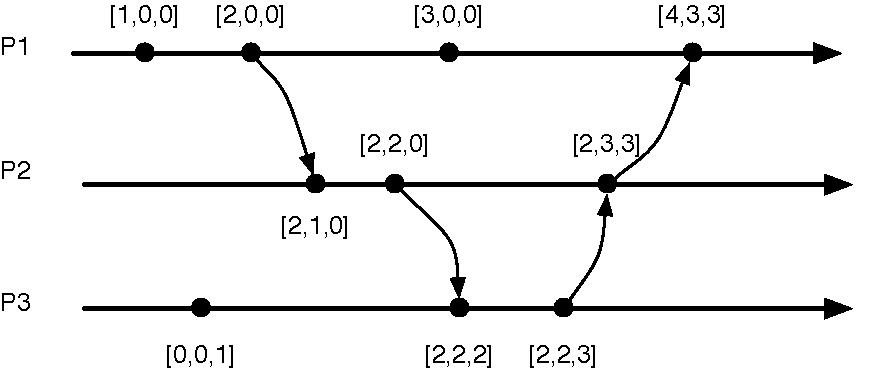
\includegraphics[width=\textwidth]{images/vector_clocks.pdf}
  \caption{ Vector Clocks}
  \label{fig:vector_clocks}
\end{figure}

Vector Clocks are able to accurately represent the
causality relation and the partial order it defines. Given any two
distinct events $x$ and $y$:

\begin{center}
\begin{math}
	\forall(x,y):(x\rightarrow y) \Longleftrightarrow (VC_x < VC_y)
\end{math}
\end{center}
Where $VC_x < VC_y$ stands for:
\begin{center}
  \begin{math}
    (\forall k: VC_x[k] \leq VC_y[k] \wedge (\exists k : VC_x[k]< VC_y[k]))
  \end{math}
\end{center}

An important property of this mechanism is the result by Charron-Bost
\cite{charron1991concerning} proving that Vector Clocks are the most
concise characterization of causality among process events.

%%% Local Variables:
%%% mode: latex
%%% TeX-master: "../thesis"
%%% End: